\documentclass[12pt]{report}
\usepackage[utf8]{inputenc}
\usepackage{natbib}%referencing
\usepackage[left=1.0in,right=1.0in,top=.8in,bottom=.8in]{geometry}
\usepackage{float}
\usepackage{caption}
\usepackage{makecell}
\usepackage{pifont}
\linespread{1.3}
\usepackage{graphicx}%figures
\usepackage{rotating}%landscape
\usepackage{amsmath, amssymb}%math
\usepackage{titlesec} %formatting chapters
\usepackage{setspace}
\usepackage{multirow}
\usepackage{bm}
\newcommand{\pmr}[1]{\scriptsize$\pm$#1}
%\titlespacing*{<command>}{<left>}{<before-sep>}{<after-sep>}
\usepackage{hyperref}
\titlespacing*{\chapter}{-15pt}{10pt}{15pt}
\titlespacing*{\section}{0pt}{0pt}{5pt}
\titlespacing*{\subsection}{0pt}{5pt}{5pt}
\titleformat{\chapter}[hang] 
{\normalfont\huge\bfseries}{\chaptertitlename\ \thechapter.}{1em}{}
\renewcommand{\chaptername}{}
\graphicspath{{Images/}}%image folder name
%Cover page contents
\title{
{
\includegraphics[scale=.3]{logotu.jpg}}\\
\uppercase\large{
    {Tribhuvan University}\\
    {Institute of Engineering}\\
    {Pulchowk Campus}\\
    \vspace{.5cm}
    {A \\Project Report\\On\\Neural Audio Codec}\\
    \vspace{.5cm}
    {\textbf{Submitted By:}\\Subodh Baral (PUL075BCT088) \\Tapendra Pandey (PUL075BCT093) \\ Achyut Burlakoti (PUL075BCT098)\\Sijal Baral (PUL075BCT100)}\\
    \vspace{.5cm}
    {\textbf{Submitted To:}\\ Department of Electronics \& Computer engineering}\\
                }
    }
\date{Apr 29, 2023} %{Month Year}

\begin{document}
\maketitle
\pagenumbering{roman}
\setcounter{page}{2}
\chapter*{Page of Approval}
\addcontentsline{toc}{chapter}{\numberline{}Page of Approval}
\vspace{1.5cm}
\begin{center}
\uppercase{
Tribhuvan Universiy\\
Institute of Engineering\\
Pulchowk Campus\\
Department of Electronics and Computer engineering
    }
    \end{center}
\vspace{.5cm}
The undersigned certifies that they have read and recommended to the Institute of Engineering for acceptance of a project report entitled \textbf{"Neural Audio Codec"} submitted by \textbf{Subodh Baral}, \textbf{Tapendra Pandey}, \textbf{Achyut Burlakoti}, \textbf{Sijal Baral} in partial fulfillment of the requirements for the Bachelor's degree in Electronics \& Computer Engineering.\\

\vspace{1cm}
\begin{minipage}{.5\textwidth}
        \raggedright
    .............................\\
    Supervisor\\
    \textbf{Dr. Sashidhar Ram Joshi, Phd.}\\
    Professor\\
    Department of Electronics and Computer Engineering,\\
    Pulchowk Campus, IOE, TU.\\
    \end{minipage}%
    \begin{minipage}{0.5\textwidth}
    \raggedleft
    .............................\\
    Internal examiner\\
    \textbf{Person B}\\
    Assistant Professor\\
    Department of Electronics and Computer Engineering,\\
    Pulchowk Campus, IOE, TU.\\
    \end{minipage}\\
    \vspace{.8cm}
    \begin{center}
    .............................\\
    External examiner\\
    \textbf{Person C}\\
    Assistant Professor\\
    Department of Electronics and Computer Engineering,\\
    Pulchowk Campus, IOE, TU.\\
    \vspace{.6cm}
    \end{center}
\centerline{Date of approval:}
%new chapter
\chapter*{Copyright}
\addcontentsline{toc}{chapter}{\numberline{}Copyright}
The author has agreed that the Library, Department of Electronics and Computer Engineering, Pulchowk Campus, Institute of Engineering may make this report freely available for inspection. Moreover, the author has agreed that permission for extensive copying of this project report for scholarly purposes may be granted by the supervisors who supervised the project work recorded herein or, in their absence, by the Head of the Department wherein the project report was done. It is understood that the recognition will be given to the author of this report and to the Department of Electronics and Computer Engineering, Pulchowk Campus, Institute of Engineering in any use of the material of this project report. Copying or publication or the other use of this report for financial gain without approval of to the Department of Electronics and Computer Engineering, Pulchowk Campus, Institute of Engineering and author's written permission is prohibited.\\
Request for permission to copy or to make any other use of the material in this report in whole or in part should be addressed to:\\
\newline
\newline
Head\\
Department of Electronics and Computer Engineering\\
Pulchowk Campus, Institute of Engineering, TU\\
Lalitpur,Nepal.
%new chapter
\chapter*{Acknowledgments}
\addcontentsline{toc}{chapter}{\numberline{}Acknowledgements}
This work has come true with substantial effort, coordination, guidance and assistance from many people who generously helped us to undertake this study. There was a lot of moral, intellectual support of different individuals and organizations, without which it would never have been possible.\\
We are sincerely grateful to the \textbf{Department of Electronics and Computer Engineering} for allowing us to do the major project relating to our academic study.\\
In addition, we would like to express our extreme gratitude to our Supervisor \textbf{Prof. Dr. Sashidhar Ram Joshi}, Dean of IOE, for his continuous supervision, valuable suggestions and encouragement despite his busy schedule. Without his support, this work would not have been completed. \\
Also, we would like to express our heartfelt gratitude to \textbf{Rara Digital Lab Pvt. Ltd.}  for providing us with the opportunity to participate in their mentorship program. Their support and guidance were invaluable in helping us develop and execute our project. We appreciate the time and resources that they invested in us and our project.\\
We would also like to thank each other of this project group for the continuous dedication, support and coordination for the project. We would especially like to thank all our friends and seniors at the Institute of Engineering, Pulchowk for their valuable comments and suggestions at different stages of this study.\\
Last but not the least, we would like to extend our deepest appreciation to our family members.\\
Subodh Baral    (PUL075BCT088)\\
Tapendra Pandey (PUL075BCT093)\\
Achyut Burlakoti(PUL075BCT098)\\
Sijal Baral     (PUL075BCT100)\\
%new chapter
\chapter*{Abstract}
Neural audio codecs that use end-to-end approaches have gained popularity due to their ability to learn efficient audio representations through data-driven methods, without relying on handcrafted signal processing components. This research paper evaluates the performance of Neural Audio Codec in comparison to traditional audio codecs Opus and EVS in terms of audio quality and efficiency. The study highlights the limitations of existing audio codecs in leveraging the abundant data available in the audio compression pipeline and proposes deep learning-based models as a potential solution. The paper reviews recent advancements in deep learning-based audio synthesis and representation learning and explores the potential of deep learning-based audio codecs in enhancing compression efficiency. The study also addresses the limitations of existing models, including slower training times and increased memory requirements, by releasing open-source code and pre-trained models for further research and improvement. Experimental results show that our approach has comparable performance to widely used commercial codec OPUS at low bitrate, and a slight drop in performance compared to current deep learning-based frameworks but at the expense of significant improvement in speed and memory requirements. We have released our code and pre-trained models at https://github.com/AchyutBurlakoti/Neural-Audio-Compression for further research and improvement.  \\
\newline
\textbf{Keywords: Audio Compression, Deep Learning, Audio Codec, Pre-trained models}
\addcontentsline{toc}{chapter}{\numberline{}Abstract}
\tableofcontents
\addcontentsline{toc}{chapter}{\numberline{}Contents}
\listoffigures
\addcontentsline{toc}{chapter}{\numberline{}List of Figures}
\listoftables
\addcontentsline{toc}{chapter}{\numberline{}List of Tables}
\chapter*{List of Abbreviations}
\addcontentsline{toc}{chapter}{\numberline{}List of Abbreviations}
\begin{tabular}{c l}

\textbf{BPS}     &  Bits Per Second\\
\textbf{CNN}     &  Convolutional Neural Networks\\
\textbf{DCT}     & Discrete Cosine Transform\\
\textbf{DTMF}    &  Dual Tone Multi-Frequency\\
\textbf{EVS}     &  Enhanced Voice Services\\
\textbf{GAN}     &  Generative Adversarial Networks\\
\textbf{MUSHRA}  &  Multiple Stimuli with Hidden Reference and Anchor\\
\textbf{PESQ}    &  Perceptual Evaluation of Speech Quality\\
\textbf{POLQA}   &  Perceptual Objective Listening Quality Assessment\\ 
\textbf{VAEs}    &  Variational Autoencoders\\
\textbf{VQ}      &  Vector Quantizer
\end{tabular}
% Latex instruction starts here

\chapter{Introduction}
\pagenumbering{arabic}%start arabic numbering(1,2,3..) from here
\section{Background}
According to recent research, traditional audio codecs such as Opus and EVS are considered state-of-the-art codecs, as they employ different coding tools, including Linear Predictive Coding (LPC), Code-Excited Linear Prediction (CELP), and Modified Discrete Cosine Transform (MDCT), to achieve high coding efficiency, low latency, and compatibility with various content types, bitrates, and sampling rates \cite{opus_codec} \cite{evs_codec}. In this study, a subjective evaluation to compare Neural Audio Codec with Opus and EVS in terms of audio quality and performance was conducted. Current audio standards have limitations in leveraging the abundant data available in the audio compression pipeline, which can potentially enhance the prediction process for more efficient entropy coding. Existing conventional approaches \cite{opus_codec, evs_codec} employ block-based structures and rely on handcrafted modules \cite{brandenburg1999mpeg, sporer2004aac, fraunhofer1997mp3}. Although neural networks have been utilized to achieve localized improvements in audio codecs, an end-to-end model could further enhance the overall compression efficiency. Nevertheless, deep learning-based models for audio coding are still in their early stages \cite{zhang2020survey}.

Recent advancements in deep learning-based audio synthesis and representation learning \cite{biswas2020audio, van2016wavenet, kleijn2018wavenet, garbacea2019low, kalchbrenner2018efficient, oord2018parallel} have brought a significant breakthrough in audio compression. Inspired by this, several deep learning-based audio codecs have been proposed \cite{zhen2019cascaded, zeghidour2021soundstream, chorowski2019unsupervised}. These approaches exploit the powerful representation ability of neural networks that learn the optimal transformation of audio waveforms to a lower-dimensional latent space. The model is composed of two parts: the encoder, which learns the prior distribution by transforming the waveform into the latent space, and the decoder, which learns the posterior distribution by predicting the waveform from the latent variable. This enables the model to learn the distribution of audio data using both the prior and posterior probabilities, expressed as $p(x,z) = \sum_{z} p(x|z) p(z)$. Despite the improvement in compression and quantization of audio signals, these models have several limitations, including slower training times and increased memory requirements. Additionally, some of these models have closed-source code, making it difficult for others to explore the pipeline further. In this work, we aim to address these limitations by releasing our open-source code and pre-trained models at https://github.com/AchyutBurlakoti/Audio-Compression for further research and improvement.

\section{Objectives}
\begin{enumerate}
    \item Build a modern audio codec, with a neural network approach, which can compress the audio file.
\end{enumerate}

\section{Scope of the Project}
There are many existing audio compression algorithms which are performing well such as MP3, AAC, and Opus, but we believe that they can be optimized further by using state-of-the-art machine learning algorithms. \\
The current amount of audio information being transmitted over the internet shows how much dependent the world has become on the audio contents be it in the field of communication, entertainment, music production, podcasting and so on. A slight improvement in the existing audio compression algorithms can save a lot of bandwidth which is soon going to be scarce given the huge rate of inflow of internet users worldwide. By using machine learning algorithms, we can potentially achieve higher compression ratios without compromising the audio quality, which can result in significant bandwidth savings and improved user experience.
\chapter{Theoretical Background}

\begin{figure}[H]
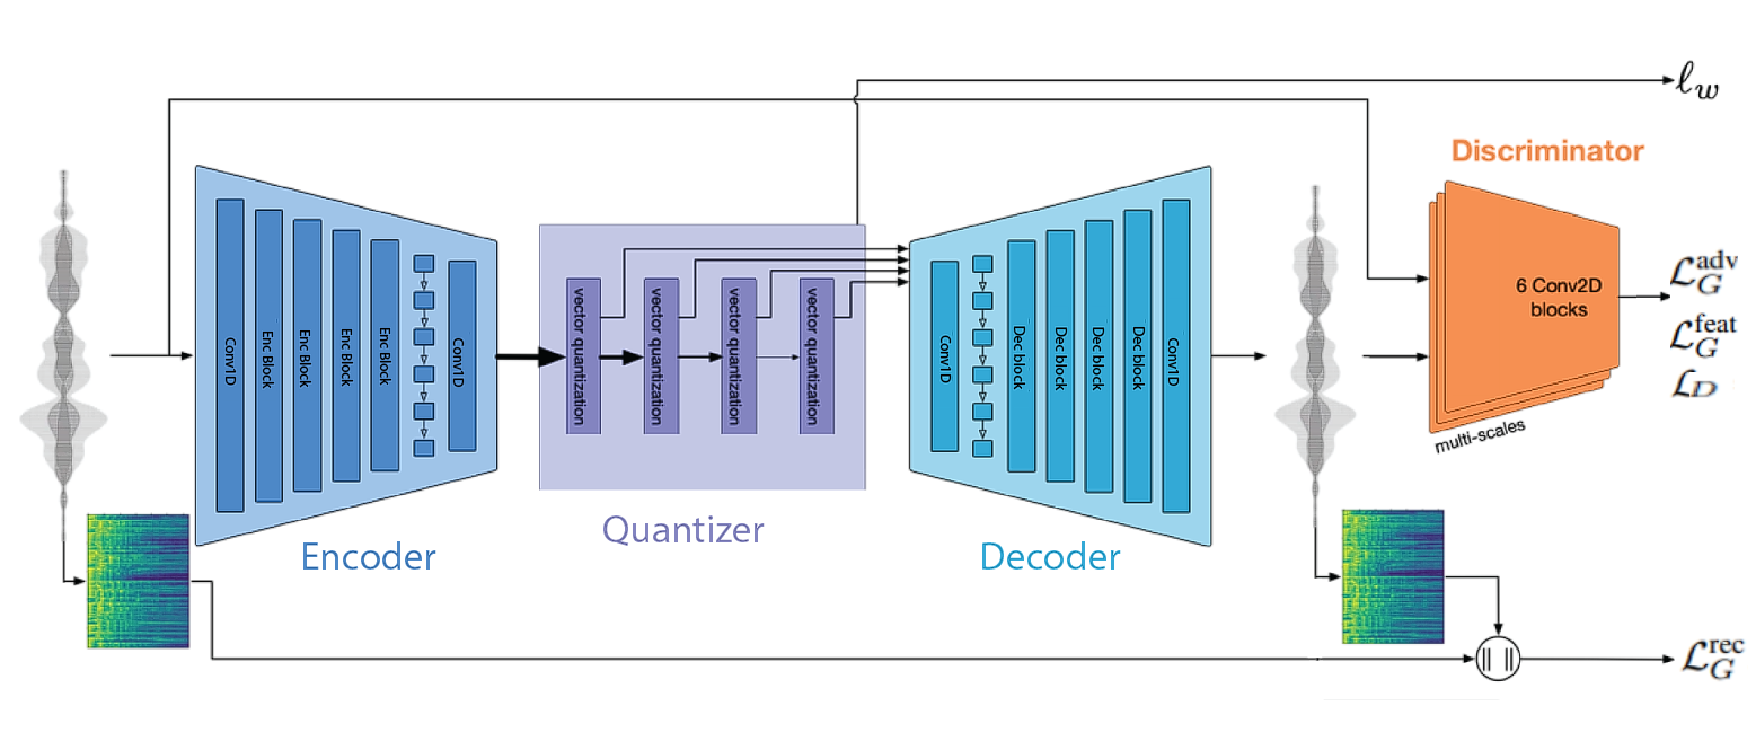
\includegraphics[width=1\textwidth]{Images/encoderdecoder.pdf}
\caption{Encoder and Decoder Model Architecture}
\end{figure}

\section{Overview of Audio Compression}
Audio compression techniques aim to reduce the amount of data needed to represent an audio signal while maintaining its perceived quality. There are two main types: lossless and lossy. Lossless compression algorithms use redundancies to achieve compression without any loss of information, while lossy algorithms discard less perceptually important information. Popular lossy formats include MP3, AAC, and Ogg Vorbis, which use psychoacoustic modeling and transform coding. Lossless formats such as FLAC and ALAC exploit the statistical properties of the audio signal without discarding any information. \\\\
\textbf{Encoder}\\
An encoder is an architecture that transforms input data into a compressed, lower-dimensional representation called a "code" or "embedding."  The encoder typically consists of multiple layers of neurons that perform non-linear transformations on the input data. These transformations progressively reduce the dimensionality of the input data, resulting in a compressed representation. \\\\\\
\textbf{Quantization}\\
Quantization is a fundamental process in data compression, and its main job is to discretize a continuous latent space by preparing a codebook. In audio and image compression, quantization is commonly used to represent high-dimensional data with lower-dimensional embeddings. The quantizer prepares the codebook for these embeddings, allowing us to store the index of their nearest neighbor in the codebook. This process is called vector quantization, and it involves grouping similar embeddings together into clusters. The codebook consists of the centroid of each cluster, which is represented by a discrete symbol. \\\\
\textbf{Decoder}\\
Decoder is multi-layered neural architecture that takes a compressed, low-dimensional representation of the input data  generated by an encoder and transforms it back into a high-dimensional output representation that can be used for tasks such as reconstruction, classification, or generation. \\\\
\textbf{Discriminator}\\
In the context of audio synthesis, a discriminator is a neural network that is trained to distinguish between real and synthetic audio signals. The discriminator is a key component of generative adversarial networks (GANs), a type of deep learning model that is widely used for audio synthesis. The discriminator is trained to learn the characteristics of real audio signals and differentiate them from synthesized signals generated by the generator network. By doing so, it provides feedback to the generator network on how to improve the quality of the synthesized audio. 
\section{Vector Quantization}
The signal processing method known as vector quantization (VQ) permits the modeling of probability density functions through the distribution of prototype vectors. Its initial application
was for data compression. It divides a big collection of points (vectors) into groups that each include roughly the same number of points that are nearest to them.
\section{DCT}
The Discrete Cosine Transform (DCT) is a transformation method commonly used in signal processing and data compression. It represents a set of finite data points as a combination of cosine functions oscillating at various frequencies. The utilization of cosine functions instead of sine functions is crucial for compression because it requires fewer cosine functions to approximate a typical signal. However, for differential equations, the use of cosines indicates a specific selection of boundary conditions.
For two dimensional signals, DCT can be represented mathematically as:
$$X_{u,v} = \frac{2}{N} \sum_{x=0}^{N-1} \sum_{y=0}^{N-1} x_{x,y} \cos \left[ \frac{\pi}{N} \left(x + \frac{1}{2} \right) u \right] \cos \left[ \frac{\pi}{N} \left(y + \frac{1}{2} \right) v \right]$$

where $0 \leq u,v < N$ are the frequency indices, and $x_{x,y}$ is the pixel value of the input signal at location $(x,y)$.
\section{CNN}
A Convolutional Neural Network (CNN) consists of an input and an output layer, as well as several hidden layers. The hidden layers in a CNN usually comprise a sequence of convolutional layers that perform dot product or multiplication. The activation function employed is typically a RELU layer, followed by further convolutional layers such as pooling, fully connected and normalization layers, collectively referred to as hidden layers because their inputs and outputs are masked by the activation function and final convolution.

Although these layers are commonly called convolutions, this is only a convention. In reality, mathematically, they perform a sliding dot product or cross-correlation. This has an impact on the matrix indices, influencing how the weight is calculated at a particular index point.\\


\begin{figure}[H]
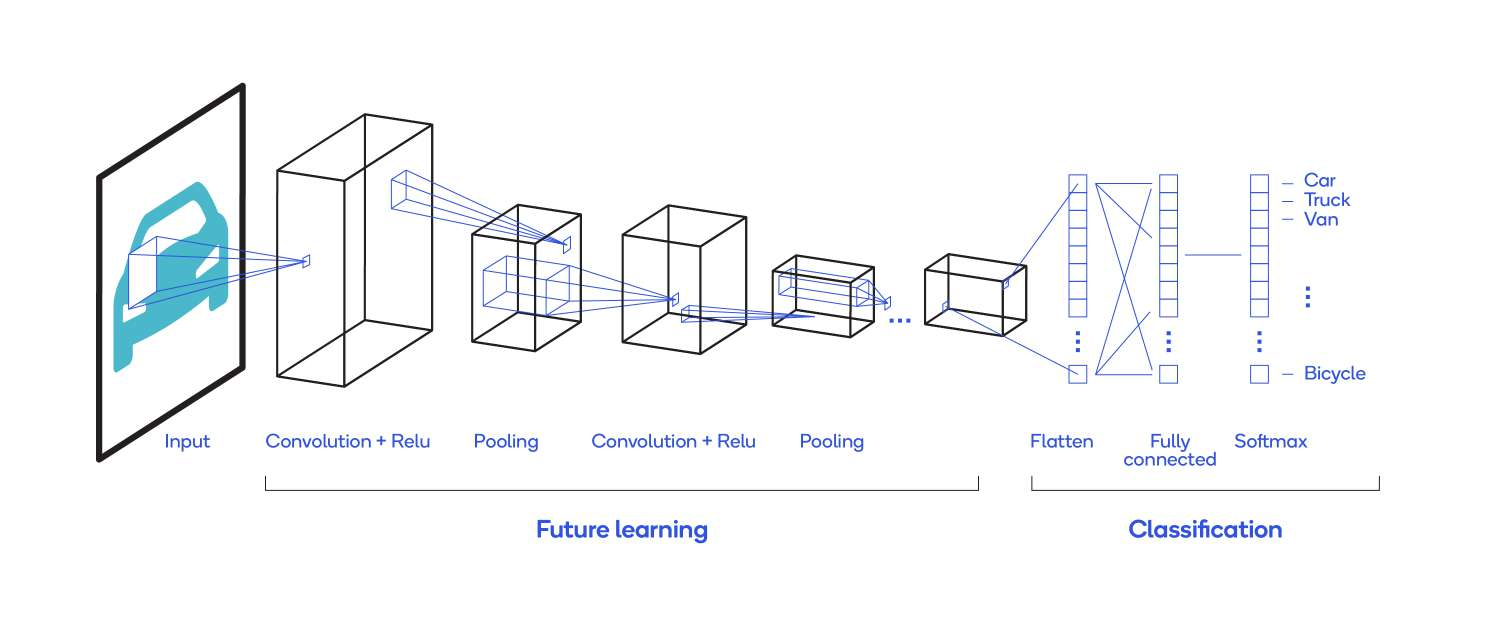
\includegraphics[width=0.9\textwidth]{Images/cnn.pdf}
\caption{CNN architecture.}
\end{figure}


\section{Auto-Encoder}
An autoencoder is an artificial neural network that operates in an unsupervised manner, and it is designed to learn how to compress and encode data efficiently. Once it has accomplished this, the network then learns how to reconstruct the original data from the compressed encoded representation, such that the final representation is as close to the original input as possible. Autoencoders are capable of transforming high-dimensional data into a more compact code representation, which can be reconstructed back to the original version with minimal or no differences. The autoencoder is made up of four major components: the encoder, the bottleneck, the decoder, and the reconstruction loss.\\

\begin{figure}[H]
\centering
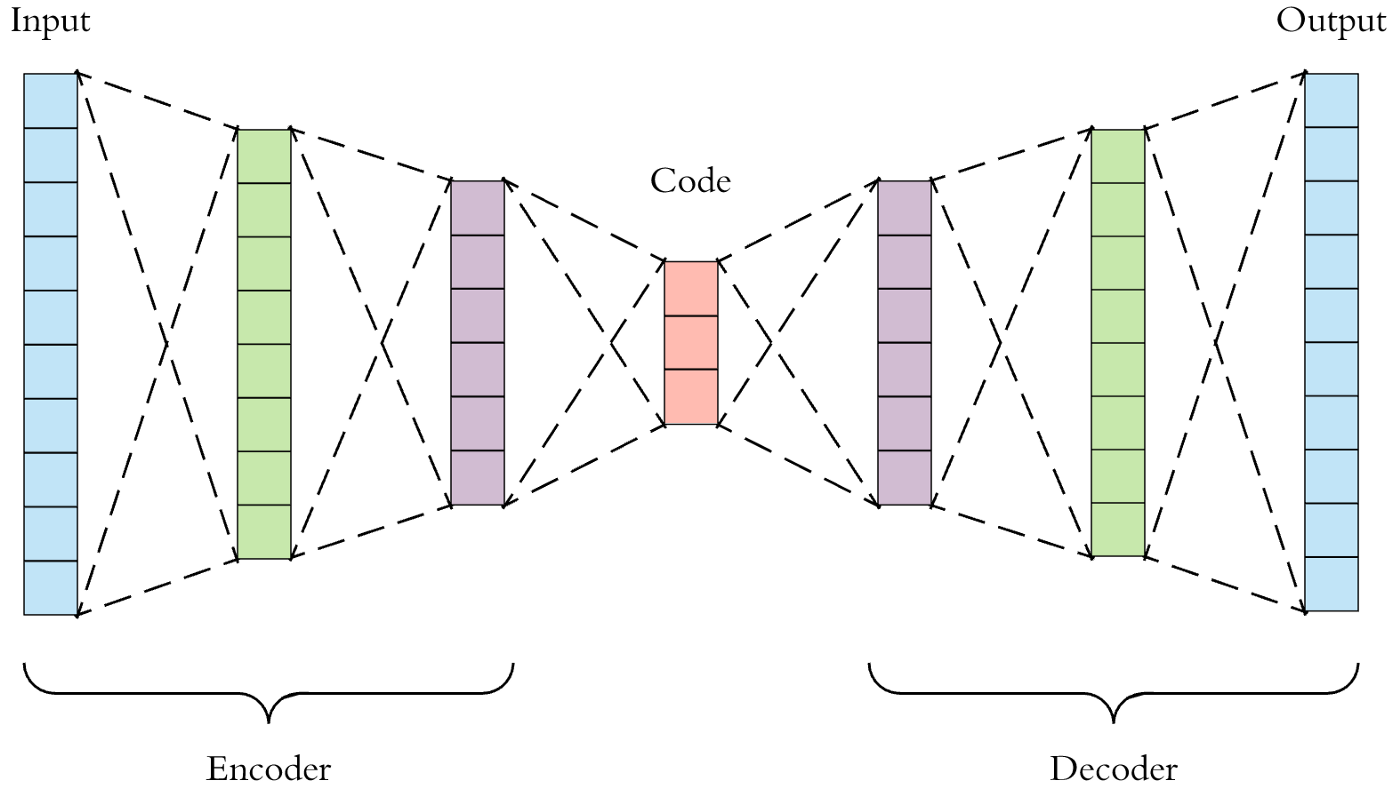
\includegraphics[width=0.5\textwidth]{Images/autoencoder.png}
\caption{Auto Encoder}
\end{figure}

\section{Variational AutoEndcoder}
A variational autoencoder (VAE), is an artificial neural network architecture introduced by Diederik P. Kingma and Max Welling, belonging to the families of probabilistic graphical models and variational Bayesian methods.
Because to its similarity in architecture, variational autoencoders are frequently compared to the autoencoder model, despite having vastly different objectives and mathematical formulations. Statistical inference issues (such determining the value of one random variable from another randomly generated value) can be reformulated as statistical optimization issues using variational autoencoders (i.e find the parameter values that minimize some objective function).

\begin{figure}[H]
\centering
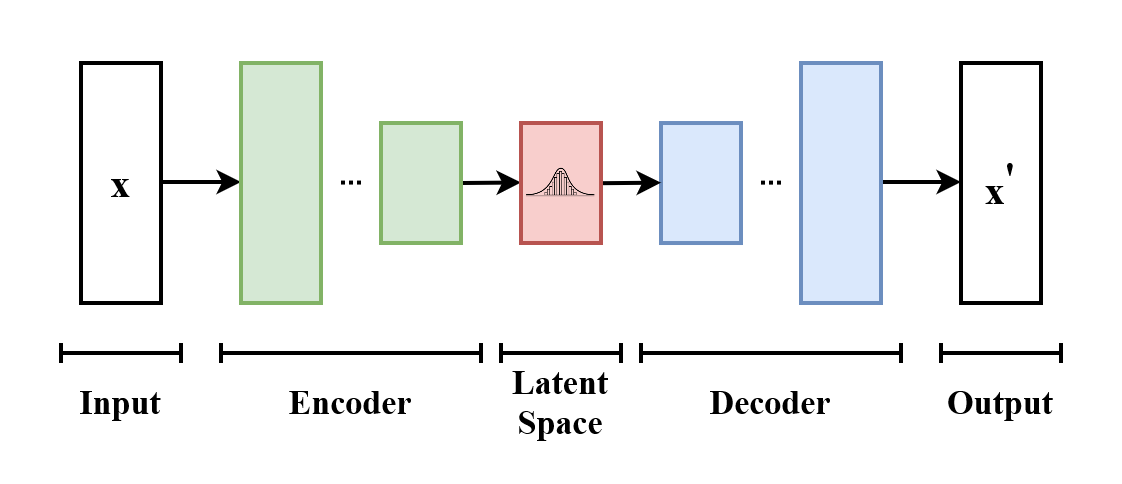
\includegraphics[width=0.6\textwidth]{Images/VAE_Basic.png}
\caption{Variational AutoEncoder}
\end{figure}

\chapter{Literature Review}
\textbf{Traditional Audio Codec}\\
Traditional audio codecs are based on block-based structures and rely on handcrafted modules for audio compression. These codecs employ subband filtering, psychoacoustic modeling, and transform coding techniques, such as the Modified Discrete Cosine Transform (MDCT), to achieve high compression ratios while maintaining perceptual audio quality.
Traditional audio codecs are based on block-based structures and rely on handcrafted modules for audio compression. These codecs employ subband filtering, psychoacoustic modeling, and transform coding techniques, such as the Modified Discrete Cosine Transform (MDCT), to achieve high compression ratios while maintaining perceptual audio quality. \\
In particular all of the audio codec explained based on this scheme. The development of audio codecs such as EVS, Opus, MPEG audio, and MP3 has enabled digital audio compression for various applications. While EVS and Opus offer high-quality compression, MPEG audio provides different levels of compression and quality, and MP3 is widely used for efficient digital audio storage and transmission. However, these traditional codecs have limitations such as limited compression efficiency, restricted quality at low bit rates, and limited support for multichannel audio. Despite these limitations, they remain widely used due to their compatibility and ease of use. \cite{opus_codec, evs_codec, brandenburg1999mpeg, fraunhofer1997mp3}.
\\\\
\textbf{Neural audio compression} \\
Neural audio codecs that use end-to-end approaches have gained popularity due to their ability to learn efficient audio representations through data-driven methods, without relying on handcrafted signal processing components. These codecs utilize autoencoder networks with quantization of hidden features, and have been applied in early works for speech coding \cite{morishima1990speech}, as well as in more recent studies, where a deep convolutional network was used for speech compression \cite{kankanahalli2018end}. While most of these works target speech coding at low bitrates, several studies have demonstrated the efficient compression of audio using neural networks. For instance, a VQ-VAE speech codec was proposed in \cite{garbacea2019low}, which operates at a bitrate of 1.6 kbps.

In recent years, several studies have proposed neural-based audio codecs that rely on quantizing the latent space prior to decoding \cite{skoglund2019waveform, valin2019neural, garbacea2019vector, lim2020high, kleijn2018straight, kleijn2021deep, jayashankar2022role, jiang2022new}. One approach, used by Valin and Skoglund, involved conditioning an LPCNet vocoder on hand-crafted features and a uniform quantizer \cite{valin2019neural}. Meanwhile, Gârbacea et al. conditioned a WaveNet model on discrete units obtained from a VQ-VAE model \cite{garbacea2019vector}. Other approaches have included feeding the Opus codec to a WaveNet in order to improve perceptual quality \cite{skoglund2019waveform}, using a vector quantization layer applied over the latent representation in an auto-encoder \cite{jayashankar2022role, jiang2022new}, and using Gumbel-Softmax for representation quantization. 

The SoundStream model developed by Zeghidour et al. is a notable example of this type of work. This model uses a fully convolutional encoder-decoder architecture with Residual Vector Quantization layers, and it is optimized using both reconstruction loss and adversarial perceptual losses \cite{zeghidour2021soundstream}. Although there are some variations in the specific methods used in each of these studies, the overall trend towards neural-based audio codecs with quantized latent spaces is clear. In most recent paper, Alexandre et al. proposed a method for high-fidelity neural audio compression using a single multiscale spectrogram adversary for efficient training and high-quality sample production, coupled with Transformer models for up to 40\% compression rates, all while maintaining real-time performance for entropy coding. \cite{defossez2022high} \\\\
\textbf{Audio Synthesis} \\
Recent studies have demonstrated that relying solely on reconstruction to generate audio can lead to the presence of noise in the output \cite{fang2020vq}. To mitigate this issue, researchers have incorporated discriminators to improve the distribution of input data approximated by the generator, resulting in reduced noise in the synthesized audio \cite{donahue2019adversarial}.

In particular, the use of discriminators from generative adversarial models such as MelGAN \cite{kumar2019melgan} and HiFiGAN \cite{kwon2020hifi} has been shown to be effective in generating high-quality audio with lower computational complexity. These models employ multi-scale waveform discriminators to enhance the quality of the synthesized waveform from the decoder \cite{kumar2019melgan}. The use of discriminators has thus emerged as a promising approach to generate high-quality audio \cite{kwon2020hifi}.
\\
\chapter{Methodology}

\begin{figure}[H]
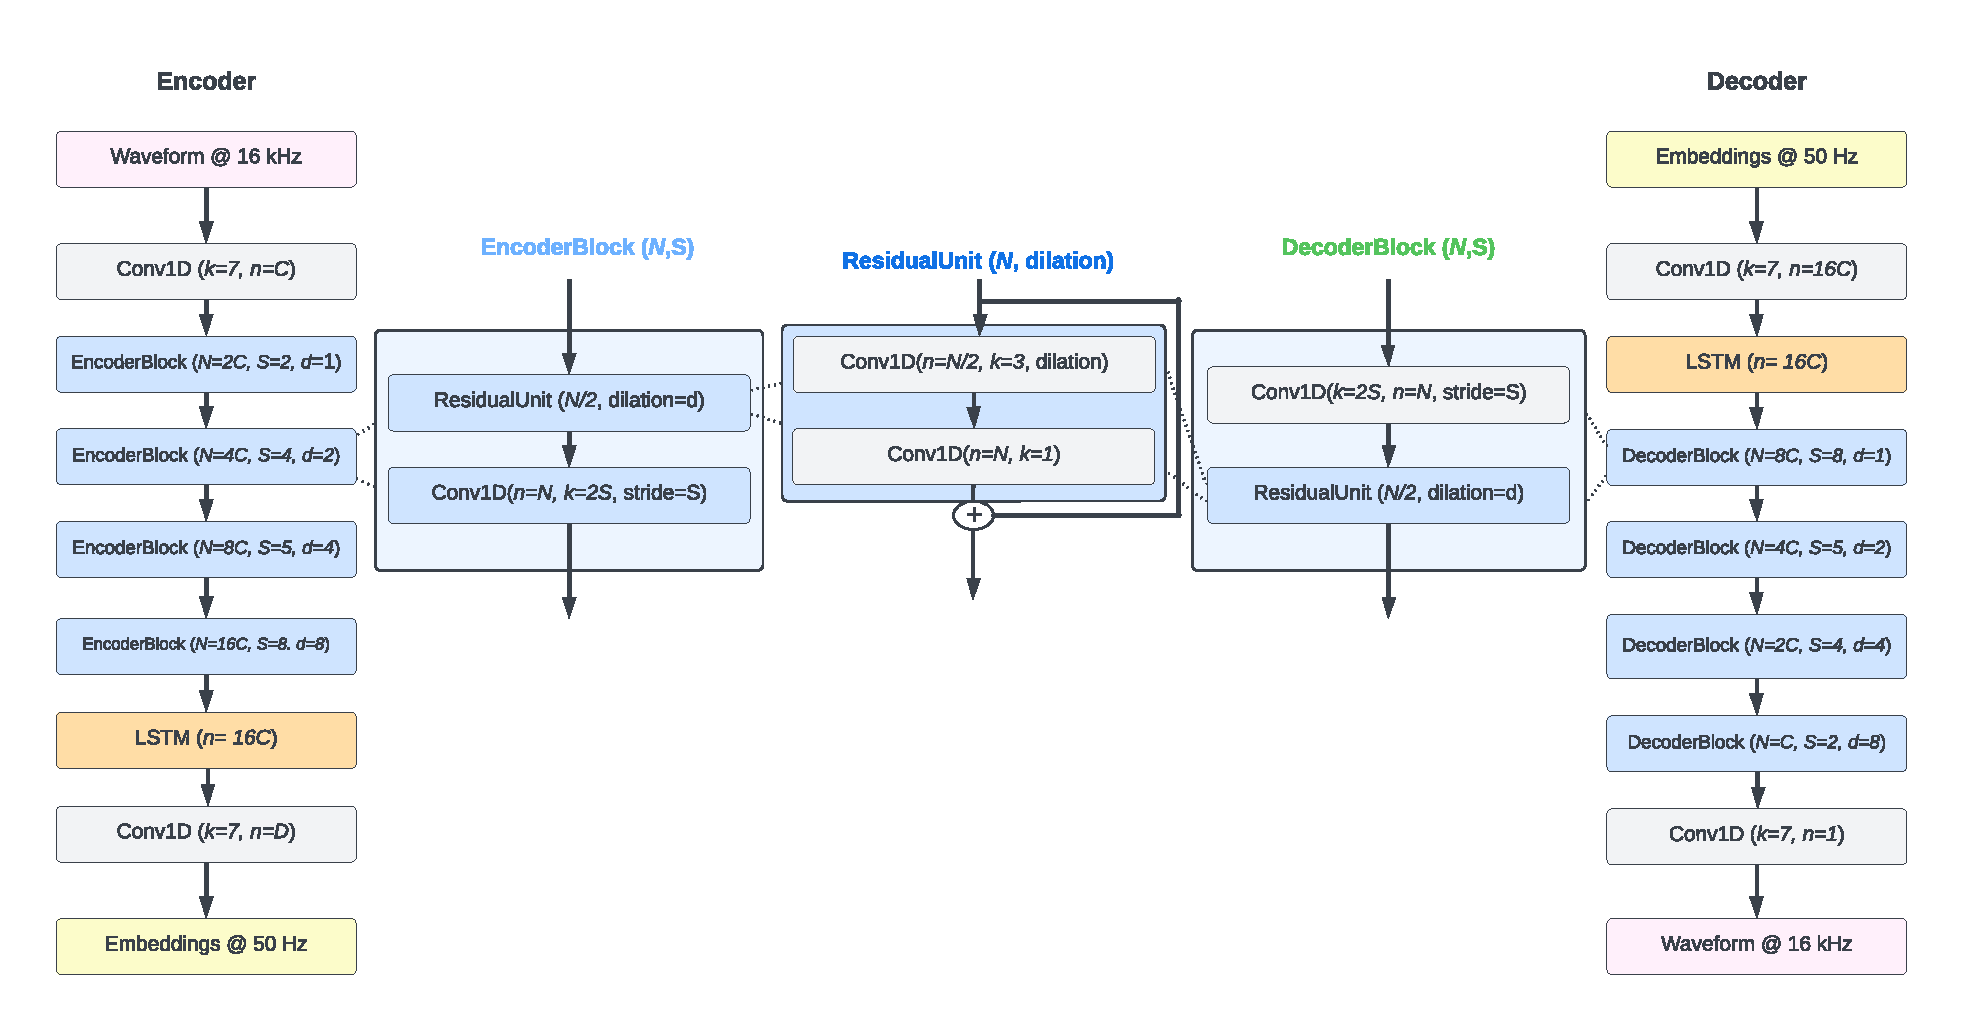
\includegraphics[width=1.07\textwidth]{Images/ED_4.pdf}
\caption{Encoder and Decoder Model Architecture}
\end{figure}

\section{Encoder Architecture} 
The encoder structure, as depicted in Figure 4.1, follows the same format as that of the SEANet encoder described in \cite{defossez2022high, tagliasacchi2020seanet}. It comprises a 1D convolution layer with $C_{enc}$ channels, followed by $B_{enc}$ encoder blocks, each with dilated convolutions at varying dilation rates of 1, 2, 4, and 8. The encoder block contains one residual block with a matching dilation, followed by a down-sampling layer in the form of a strided convolution. The number of channels is doubled when down-sampling, starting from $C_{enc}$. The embeddings are dimensionally reduced to $D$ using a final 1D convolution layer with a 7-length kernel and a stride of 1. All convolutions are causal to ensure real-time inference, with padding applied only to the past in both training and offline inference. No normalization is applied, and the ELU activation function is used \cite{clevert2015fast}.

The temporal resampling ratio between the input waveform and the embeddings is determined by the number of encoder blocks, $B_{enc}$, and the corresponding striding sequence. For example, when $B_{enc}$=4 and using strides of (2, 4, 5, 8), one embedding is generated for every $M=320$ input samples, where $M$ is calculated as (2 . 4 . 5 . 8). Thus, the encoder output, $enc(x)$, is in $\mathbb{R}^{S \times D}$, with $S = T / M$.

This description is based on \cite{opus_codec, evs_codec} and explains the encoder architecture employed in the paper.



\section{Quantizer}
The quantizer's objective is to compress the encoder's output, $enc(x)$, to a specific bitrate, $R$, expressed in bits per second (bps). Joint training of the quantizer, encoder, and decoder is necessary for an end-to-end approach, which can be achieved by backpropagation. The vector quantizer (VQ) proposed for VQ-VAE in \cite{oord2017neural} satisfies this requirement. It generates a codebook of $N$ vectors to encode each D-dimensional frame of $enc(x)$. Next, $enc(x)$ is mapped to a sequence of one-hot vectors of shape $S$ × $N$, which requires $\log_2$ $N$ bits for representation.\\\\
\textbf{Limitation of Vector Quantization} \\
To illustrate, suppose we have a codec with a target bitrate of $R$ = 3000 bps. With a striding factor of $M$ = 320, one second of audio at a sampling rate of $f_{s}$ = 16000 Hz is represented by S = 50 frames at the encoder output. Each frame is assigned r = 3000 / 50 = 60 bits, given the target bitrate of R. If we were to use a simple vector quantizer, we would need to store a codebook comprising $N$ = $2^{60}$ vectors, which is not feasible due to its impractical size.\\\\
\textbf{Residual Vector Quantizer}\\
In order to address this issue, we have decided to utilize a Residual Vector Quantizer, which is also known as a multi-stage vector quantizer. This technique involves incorporating $N_{q}$ layers of VQ in a specific manner. Initially, the unquantized input vector is processed through a first VQ to derive quantization residuals. Subsequently, the residuals are subject to iterative quantization by means of a sequence of additional $N_{q}$ - 1 vector quantizers, following the guidelines presented in Algorithm 1. The total rate budget is distributed uniformly across all VQs, whereby $r_i$ = $r$/$N_q$ = $\log_2$ $N$. If, for instance, $N_q$ = 6, each quantizer would make use of a codebook consisting of $N$ = 2$^{r/N_q}$ = 2$^{60/6}$ = 1024. By manipulating the $N_q$ parameter, one can balance the computational complexity and coding efficiency to meet a desired target rate budget $r$.
\\
\begin{figure}[H]
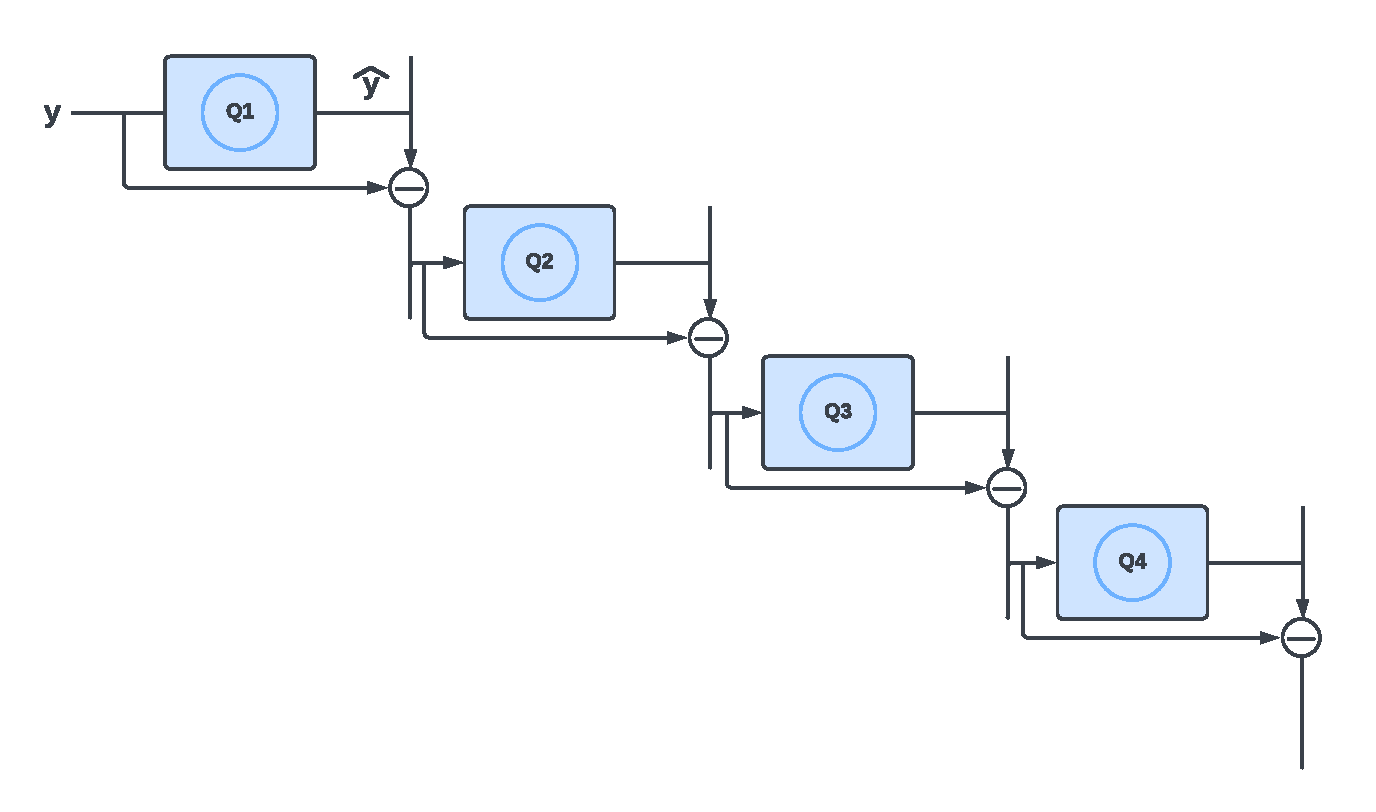
\includegraphics[width=1\textwidth]{Images/rvq.pdf}
\caption{Residual Vector Quantizer (for $N_q$=4)}
\end{figure}
\textbf{}
% Algorithm for RVQ %
\begin{tabular}{l}
\hline \textbf{Algorithm 1:} Residual Vector Quantization \\
\hline \textbf{Input:} $y=\operatorname{enc}(x)$ the output of the encoder, vector \\
$\quad$ quantizers $Q_i$ for $i=1 . . N_q$ \\
\textbf{Output:} the quantized $\hat{y}$ \\
$\hat{y} \leftarrow 0.0$ \\
residual $\leftarrow y$ \\
\textbf{for} $i=1$ to $N_q$ \textbf{do} \\
\hspace{1.05cm}$\begin{array}{l}\hat{y}+=Q_i(\text { residual }) \\
\text {residual }-=Q_i(\text { residual })\end{array}$\\
\textbf{return} $\hat{y}$\\
\hline
\end{tabular}

\textbf{}\\\\
\textbf{Scalable Bitrate} \\
To allow for scalability in bitrate, quantizer dropout is utilized, and residual vector quantization serves as a useful framework for controlling bitrate. The bitrate is determined by the number of VQ layers, $N_q$, given a fixed codebook size, N, for each layer. In principle, a different model should be trained for each target bitrate, as the vector quantizers are trained jointly with the encoder/decoder. However, it is much more practical to have a single model that can scale to several target bitrates, as it reduces the memory required to store model parameters on both the encoder and decoder side.

To create a model capable of handling multiple bitrates, we make a modification to Algorithm 1. When processing each input example, we randomly sample a value for nq from the range [1; $N_q$] and only use quantizers $Q_i$ for i = 1 . . . $n_q$. This is similar to applying structured dropout to the quantization layers. As a result, the model is trained to encode and decode audio at all target bitrates within the range $n_q$ = 1 . . . $N_q$. During the inference phase, we select the value of nq based on the desired bitrate. By implementing this approach, we can create a model that is more memory-efficient than having to train separate models for each target bitrate.

The additive composition of the outputs of each VQ layer progressively refines the quantized embeddings, while keeping the same shape. Hence, no architectural changes are needed in neither the encoder nor the decoder to accommodate different bitrates
\section{Decoder Architecture}
The design of the decoder architecture is similar to that of the encoder architecture, as shown in Figure 3. The decoder block consists of a transposed convolution for up-sampling, followed by residual units, which is identical to the encoder block. We use the reverse order of strides as the encoder to reconstruct a waveform with the same resolution as the input waveform. During up-sampling, the number of channels is halved, and the last decoder block generates $C_{dec}$ channels. A final 1D convolution layer, with a kernel size of 7 and stride 1, with only one filter, is used to project the embeddings back to the waveform domain and produce $\hat{x}$. The same number of channels in both the encoder and decoder is controlled by the same parameter, $C_{enc}$ = $C_{dec}$ = $C$, as illustrated in Figure 4.1.
\section{Discriminator Architecture}
In line with Wang et al. \cite{wang2018high}, we utilize a multi-scale architecture that includes three discriminators (D1, D2, D3) with the same network structure but differing audio scales. D1 operates on raw audio scale, while D2 and D3 operate on raw audio downsampled by a factor of 2 and 4, respectively. The downsampling is achieved using strided average pooling with a kernel size of 4. The use of multiple discriminators at different scales is justified by the fact that audio has different structures at various levels. This structure is supported by an inductive bias that each discriminator learns features for various frequency ranges of the audio. For instance, the discriminator operating on downsampled audio lacks access to high-frequency components; thus, it is inclined to learn discriminative features based on low-frequency components only.

\begin{figure}[H]
\centering
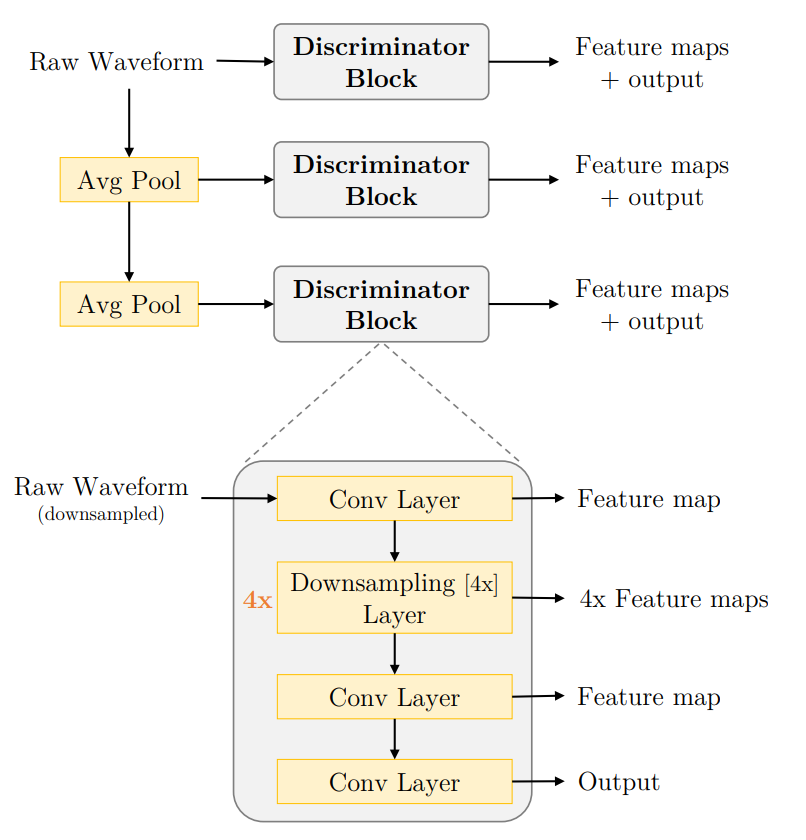
\includegraphics[width=0.5\textwidth]{Images/discriminator.png}
\caption{Discriminator}
\end{figure}

\section{Regularization}
\textbf{Dropout Regularization}\\
Dropout is a popular regularization technique used in deep learning to prevent overfitting of the model. By randomly dropping out some of the neurons in a neural network during training, dropout forces the network to learn redundant representations, which makes it more robust and less likely to overfit. The dropout technique was introduced by Srivastava et al.\cite{srivastava2014dropout} in their 2014 paper "Dropout: A Simple Way to Prevent Neural Networks from Overfitting". Dropout can be applied to various types of neural network architectures, including fully connected networks, convolutional neural networks (CNNs), and recurrent neural networks (RNNs). To incorporate dropout in a residual block, a dropout layer can be added after the final activation function in the block, before the output is added to the input. The dropout layer can have a dropout rate of p, which determines the fraction of neurons that are randomly dropped out. The value of p should be chosen based on the complexity of the model and the size of the training dataset. In their paper "Identity Mappings in Deep Residual Networks", He et al. \cite{he2016identity} showed that using dropout in residual networks can further improve the generalization performance of the model, especially when combined with other regularization techniques. Overall, dropout is a simple and effective regularization technique that can be used to improve the generalization performance of deep learning models, including residual networks.\\\\
\textbf{Time Jitter Regularization} \\
Our goal is for the model to acquire a speech representation that matches the phonetic content that changes gradually within an utterance, which is a mostly steady signal that may suddenly change at the boundaries of phonemes.
To avoid co-adaptation of latent vectors, a time-jitter regularizer inspired by dropout \cite{srivastava2014dropout} was employed in the vq-speech model\cite{chorowski2019unsupervised}. During training, a latent vector can replace one or both of its adjacent vectors, similar to dropout, which prevents the model from depending on consistency across groups of tokens. Furthermore, this regularization encourages stability in latent representations over time. A latent vector extracted at a specific time step should also be beneficial at time steps immediately preceding or following it.
\section{Training Objectives}
\textbf{Reconstruction Loss}\\
In this paper, we adapt a frame-level auxiliary loss between the original and the generated speech as in \cite{yamamoto2019probability}. The Loss functions that are correlated with perceptual audio quality should be used to train the model.
$$
\mathcal{L}_{G}^{rec}=\lambda_{\mathrm{1}} \mathcal{L}_{\mathrm{SC}}(\boldsymbol{x}, \hat{\boldsymbol{x}})+\lambda_{\mathrm{2}} \mathcal{L}_{\mathrm{logMAG}}(\boldsymbol{x}, \hat{\boldsymbol{x}})+\lambda_{\mathrm{3}} \mathcal{L}_{\mathrm{linMAG}}(\boldsymbol{x}, \hat{\boldsymbol{x}}),                   
$$

where $\boldsymbol{x}$ and $\hat{\boldsymbol{x}}$ denote the target and the estimated audio signal. \\
$\lambda_{1}$, $\lambda_{2}$ and $\lambda_{3}$ denotes the weight coefficient to balance losses, spectral convergence ($\mathcal{L}_{SC}$), log STFT manginuted loss ($\mathcal{L}_{logMAG}$) and linear STFT magnitude loss ($\mathcal{L}_{linMAG}$), which is defined as follows:
$$
\mathcal{L}_{\mathrm{SC}}(\boldsymbol{x}, \hat{\boldsymbol{x}})=\frac{\||\operatorname{STFT}(\boldsymbol{x})|-|\operatorname{STFT}(\hat{\boldsymbol{x}})|\|_F}{\||\operatorname{STFT}(\boldsymbol{x})|\|_F}
$$
$$
\mathcal{L}_{\mathrm{logMAG}}(\boldsymbol{x}, \hat{\boldsymbol{x}})=\|\log |\operatorname{STFT}(\boldsymbol{x})|-\log |\operatorname{STFT}(\hat{\boldsymbol{x}})|\|_1,
$$
$$
\mathcal{L}_{\mathrm{linMAG}}(\boldsymbol{x}, \hat{\boldsymbol{x}})=\| |\operatorname{STFT}(\boldsymbol{x})|- |\operatorname{STFT}(\hat{\boldsymbol{x}})|\|_1,
$$
\textbf{Discriminative and Generator Loss}\\
The objective of the adversarial loss is to enhance the visual appeal of the output. It is described as a hinge loss that is applied to the discriminator's logits, and it is averaged over multiple discriminators and time. To be more precise, let k  $\in \big\{0,. . . , k\big\}$ be used to identify individual discriminators, where k = 0 refers to the STFT-based discriminator, and k $\in \big\{1, . . . , K\big\}$ represents the various resolutions of the waveform-based discriminator (we use K = 3 in this study). Let $T_k$ be the number of logits produced by the $k$-th discriminator over the time dimension. The goal is for the discriminator to classify original versus decoded audio by minimizing the loss.

$$
\mathcal{L}_D = E_{x} [\frac{1}{K} \sum_{k}\frac{1}{T_{k}}max(0, 1-D_{k,t}(x))] + E_{x} [\frac{1}{K} \sum_{k}\frac{1}{T_{k}}max(0, 1+D_{k,t}(G(x)))]
$$
while the adversarial loss for the generator is
$$
\mathcal{L}_G^{adv} = E_{x} [\frac{1}{K} \sum_{k, t}\frac{1}{T_{k}}max(0, 1-D_{k,t}(G(x)))]
$$

The feature loss is computed by taking the average absolute difference between the discriminator’s internal layer outputs for the generated audio and those for the corresponding target audio.

$$
\mathcal{L}_G^{feat} = E_{x} [\frac{1}{KL} \sum_{k,l}\frac{1}{T_{k,l}}\sum_{t}\lvert D_{k,t}^{(l)}(x)-D_{k,t}^{(l)}(G(x)) \lvert] 
$$

where $\mathcal{L}$ is the number of internal layers, $D_{k,l}^{(l)} (l\in\big\{1,...,L\big\})$ is the $t$-the output of layer $l$ of discriminator $k$, and $T_{k,l}$ denotes the length of the layer in the time dimension.\\\\
\textbf{VQ commitment loss}\\
We add a commitment loss $\mathcal{L}_w$ between the output of
the encoder, and its quantized value, with no gradient being computed for the quantized value. For each residual step c $\in \big\{0,. . . , C\big\}$ (with C depending on the bandwidth target for the current batch), noting $z_{c}$ the
current residual and $q_{c}$($z_{c}$) the nearest entry in the corresponding codebook, we define $\mathcal{L}_w$ as
$$
\mathcal{L}_w=\sum_{c=1}^C\left\|\boldsymbol{z}_c-q_c\left(\boldsymbol{z}_c\right)\right\|_2^2
$$
\textbf{Total Generator loss} \\
$$
\mathcal{L}_G=\lambda_{\text {adv }} \mathcal{L}_G^{\text {adv }}+\lambda_{\text {feat }} \cdot \mathcal{L}_G^{\text {feat }}+\lambda_{\text {rec }} \cdot \mathcal{L}_G^{\text {rec }}
$$
\section{Implementation Details}
We trained the model for 3000 epochs, with epoch being 5,000 updates with the Adam optimizer with an initial learning rate of 3e$\pm$4 for generator and 1e$\pm$4 for the discriminator and default parameters $\beta{_1}$ = 0.9 and $\beta{_2}$ = 0.999 for optimization. The mini-batch size is set to 10 and the whole system is
implemented in PyTorch. We set the $\lambda_{1}$=1, $\lambda_{2}$=1 and $\lambda_{3}$=0 for reconstruction loss and  $\lambda_{\text {adv}}$=1, $\lambda_{\text {feat}}$=100 and $\lambda_{\text {rec}}$=1 to scale adversarial, feature and reconstruction losses for generator loss.
\chapter{Evaluation Setup}
\section{Dataset}
We train our model on three types of audio content: clean speech, noisy speech, and music, all at a 16 kHz sampling rate. The audio data from \cite{muscan} were further processed using ffmpeg to transform the given data into a suitable representation i.e. sampling frequency of 16 kHz with 16 bits per sample. In total 20,000 audio files were used to train the model with 7,500 clean speech, 7,500 noisy speech, and 5,000 music. For validation in total 60 audio files were used with 20 from each clean speech, noisy speech, and music.

\section{Evaluation Metric}
To evaluate our model, we conducted both subjective and objective evaluations of the results. For subjective evaluation the MUSHRA\cite{itu-r-bs1534-1} test is used, it involves presenting a listener with several audio stimuli, which can be different versions of the same audio signal, or different audio signals altogether. One of the stimuli is designated as the "anchor", which is a high-quality reference signal that serves as a benchmark for comparison. The listener is asked to rate the quality of each stimulus using a numerical scale, typically ranging from 0 to 100, where 0 represents the worst possible quality and 100 represents the best. Ratings were screened to exclude noisy data. For objective evaluation of the model, SCALE-INVARIANT SIGNAL-TO-NOISE RATIO was used. While SI-SNR is primarily used in speech separation and speech enhancement applications, it can also be used as a metric for evaluating audio codecs.

\section{Baselines}
Opus and EVS are set as baselines for comparison with traditional audio codecs. Opus \cite{opus_codec} is a popular speech and audio codec widely used for internet communication applications, such as Zoom, Microsoft Teams, and Google Meet, as well as for streaming on YouTube. It supports a range of signal bandwidths from 4 kHz to 24 kHz and bitrates from 6 kbps to 510 kbps. Another versatile codec used for Voice over LTE (VoLTE) is Enhanced Voice Services (EVS) \cite{evs_codec}, which operates at multiple signal bandwidths from 4 kHz to 20 kHz and bitrates from 5.9 kbps to 128 kbps. Both codecs serve as baselines for comparison with our model, which is designed to enhance audio quality. For comparison with neural audio codecs, Meta's Encodec \cite{defossez2022high} and Google's SoundStream \cite{zeghidour2021soundstream} are used.

\chapter{Result and Discussion}
The developed audio codec was compared with the baselines in different categories which are explained below:-\\\\
\textbf{Subjective and Objective Evaluation} \\
An experiment was conducted using headphones and 50 English speakers to subjectively evaluate the performance of our codec. The evaluation dataset comprised 20 samples of clean, noisy, reverberant speech, and music. Each sample was rated using a crowd-sourced methodology inspired by MUSHRA. The results of the subjective evaluation are shown in Table \ref{tab:intermodelcomp}. It can be observed that our codec outperformed traditional audio codec(OPUS) at low bitrates. However, our codec was unable to surpass neural audio codecs like Soundstream (by Google) and Encodec (by Meta). For comparison with the Baseline, our model with a high MUSHRA score was selected and the performance of our model with different additional components can be seen in Table \ref{tab:ourmodelcomp}. In order to further improve the quality of the decompressed audio, a Discriminator was used to remove the artifacts from the reconstructed audio signal as shown in Table \ref{tab:disccomp}. Table \ref{tab:snrcomp} shows that our model's SNR score is far less than others which makes the MUSHRA the main evaluation metric for the analysis of our model. The poor SI-SNR score is mainly because it is primarily used in speech separation and speech enhancement applications.\\\\
\textbf{Openness} \\
Also, there are no fully open-source neural audio codecs available on the internet. Table \ref{tab:opennesscomp} shows the open-source state of different neural audio codecs on the internet. 
 \\\\
\begin{table}[H]
\centering
\captionsetup{singlelinecheck=false, font=small}
\caption{MUSHRA($\uparrow$) scores of our models with different additional components. Performance of our model with different additional components at different bitrates along with the model complexity. Here rrdb represents the Residual-in-Residual-Dense Block from \cite{kwon2020hifi} which replaces the normal residual block of the model but increases complexity and jitter is the time jitter regularization for the robustness of quantized space.}
\renewcommand{\arraystretch}{1.5}
\begin{tabular}{lcccccc}
\hline Model                              & 3 kbps    & 6 kbps    & 12 kbps    & 24 kbps    & Params   \\ 
\hline Ours                                & 15 & 32 & 35 & 38 & 6.27M  \\
Ours + lstm                                & 20 & 40 & 45 & 50 & 14.67M  \\
\textbf{Ours + lstm + dropout(0.2)}      & \textbf{25} & 40 & \textbf{52} & \textbf{55} & 14.67M  \\
Ours + lstm + dropout(0.5)               & 15 & 16 & 15 & 17 & 14.67M  \\
Ours + lstm + dropout(0.2) + rrdb        & 22 & \textbf{44} & 50 & 50 & 30.5M  \\
Ours + lstm + dropout(0.2) + jitter & 10 & 12 & 11 & 10 & 14.67M  \\
\hline
\end{tabular}
\label{tab:ourmodelcomp}
\end{table} 

\begin{table}[H]
\centering
\captionsetup{singlelinecheck=false, font=small}
\caption{MUSHRA($\uparrow$) scores our model with and without discriminator for 6 kbps.}
\renewcommand{\arraystretch}{1.5}
\begin{tabular}{lcc}
\hline Model & Speech & Music \\
\hline without disc & 29 & 32 \\
with disc & 40& 47 \\
\hline
\end{tabular}
\label{tab:disccomp}
\end{table} 

\begin{table}[H]
\centering
\captionsetup{singlelinecheck=false, font=small}
\caption{Comparision of SI-SNR($\uparrow$) scores.}
\renewcommand{\arraystretch}{1.2}
\begin{tabular}{lc}
\hline Model & Speech  \\
\hline OPUS & 2.45 \\
EVS & 1.89 \\
ENCODEC & 6.67 \\
SoundStream & 6.5 \\
Ours & 1.2 \\
\hline
\end{tabular}
\label{tab:snrcomp}
\end{table} 

\begin{table}[H]
\centering
\captionsetup{singlelinecheck=false, font=small}
\caption{Openness of different models compared to ours.}
\renewcommand{\arraystretch}{1.5}
\begin{tabular}{lcccc}
\hline Codec & Code & Model & Paper & Reusability \\
\hline SoundStream & \ding{55} & \ding{55} & \ding{51} & \ding{55} \\
ENCODEC & \ding{55} & \ding{51} & \ding{51} & \ding{55} \\
Ours & \ding{51} & \ding{51} & \ding{51} & \ding{51} \\
\hline
\end{tabular}
\label{tab:opennesscomp}
\end{table} 

\begin{table}[H]
\centering
\captionsetup{singlelinecheck=false, font=small}
\caption{MUSHRA($\uparrow$) scores comparison of our's best model from Table \ref{tab:ourmodelcomp} with different state-of-the-art traditional and neural audio codec.}
\renewcommand{\arraystretch}{1.5}
\setlength{\tabcolsep}{12pt}
\begin{tabular}{lccc}
\hline Model                            & Bandwidth    & Speech          & Music   \\ 
\hline Reference                               & -            & 95.5\pmr{1.6}  & 93.2\pmr{2.5} \\
\hline OPUS                              & 6.0 kbps     & 30.1\pmr{2.8} & 20.6\pmr{5.8} \\
OPUS                                     & 12.0 kbps     & 76.5\pmr{2.3} & 77.8\pmr{3.2} \\
\hline EVS                               & 9.6 kbps     &  84.4\pmr{2.5} & 89.9\pmr{2.3} \\
\hline Lyra-v2                           & 3.0 kbps     & 53.1\pmr{1.9} & 69.3\pmr{3.3} \\
Lyra-v2                           & 6.0 kbps     & 66.2\pmr{2.9} & 75.7\pmr{2.6} \\
\hline ENCODEC                   & 1.5 kbps     & 49.2\pmr{2.4} & 68.2\pmr{2.2} \\
ENCODEC                   & 3.0 kbps     & 67.0\pmr{1.5} & 89.6\pmr{3.1} \\
ENCODEC                   & 6.0 kbps     & 83.1\pmr{2.7} & 92.9\pmr{3.1} \\
ENCODEC                   & 12.0 kbps     & 90.6\pmr{2.6} & 91.8\pmr{2.5} \\
\hline SoundStream        & 3.0 kbps     & 67.0\pmr{1.5} & - \\
SoundStream               & 6.0 kbps     & 80.0\pmr{1.5} & - \\
SoundStream               & 12.0 kbps    & 82.0\pmr{1.5} & - \\
\hline Ours               & 3.0 kbps     & 25.0 & 30.0 \\
Ours               & 6.0 kbps     & 40.0 & 47.0 \\
Ours               & 12.0 kbps     & 50.0 & 52.0 \\
Ours               & 24.0 kbps     & 50.0 & 55.0 \\
\hline
\end{tabular}
\label{tab:intermodelcomp}
\end{table} 

\begin{figure}[H]
\centering
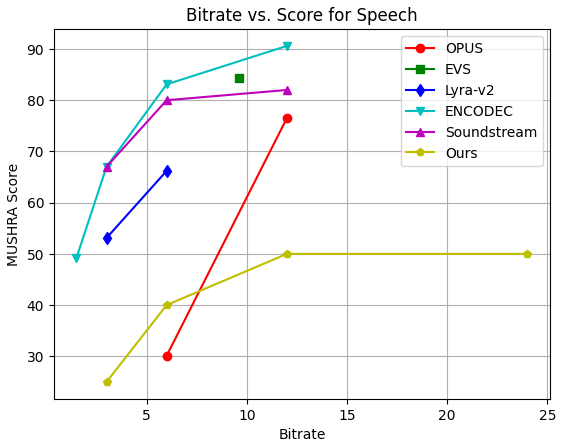
\includegraphics[width=0.6\textwidth]{Images/speechscore.png}
\caption{Ours vs state-of-art codecs for Speech}
\end{figure}

\begin{figure}[H]
\centering
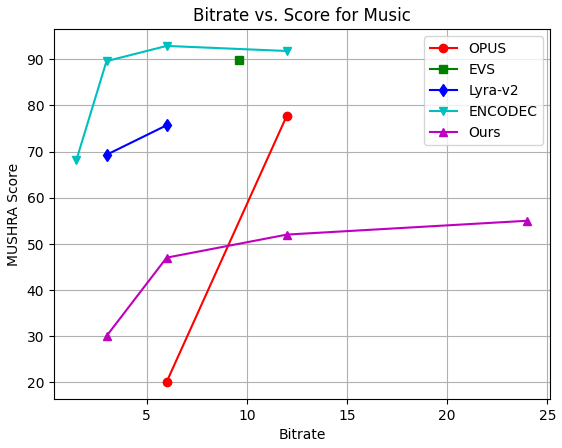
\includegraphics[width=0.6\textwidth]{Images/mucisscore.png}
\caption{Ours vs state-of-art codecs for Music}
\end{figure}

\newpage
\raggedright
\textbf{Latency and Real Time Factor} \\
Latency refers to the delay between the time an audio signal enters the codec and the time it is processed and output. In other words, it is the time it takes for the codec to encode or decode the audio signal. We profiled our model on a single thread of an intel i7-10870H CPU and Nvidia RTX 3060 GPU at 6 kbps while other models' latency and RTF values are taken from Table 5 of \cite{defossez2022high} where these models are evaluated on a single thread of a MacBook Pro 2019 CPU. The calculation of latency involves the time taken by ffmpeg to transform audio to 16-bit 16000 hz audio plus the model's encoding and decoding speed. The ffmpeg nearly takes about 6 ms to convert the audio which increases the latency of the codec.

The real-time factor is here defined as the ratio between the duration of the audio and the processing time so that it is greater than one when the method is faster than real-time. The calculation of latency and real-time factor is shown in Table \ref{tab:latencycomp}. In this analysis, our codec out-perform the other audio codec mainly due to its smaller model size. 



\begin{table}[H]
\captionsetup{singlelinecheck=false, font=small}
\caption{Latency($\downarrow$) and RTF($\uparrow$) of our model and ENCODEC, Lyra v2, SoundStream, OPUS. All models are evaluated at 6 kbps.}
\renewcommand{\arraystretch}{1.5}
\setlength{\tabcolsep}{12pt}
  \centering
  \begin{tabular}{lcrrrr}
  \hline
    & & \multicolumn{4}{c}{Real Time Factor}\\
    Model & Latency & \emph{Enc.} & \emph{Dec.}  \\
    \hline
    Lyra v2 (32 kHz) & - & 27.4 & 67.2 \\
    \hline
    ENCODEC 24 kHz & 13 ms & 9.8 & 10.4 \\
    ENCODEC 48 kHz & 1 s & 6.8 & 5.1 & \\
    \hline
    SoundStream 24 kHz & 13 ms & - & - \\
    \hline 
    OPUS  & 26.5 ms & - & - \\
    \hline
    Ours 16 kHz (cpu)  & 12 ms & 55.56 & 111.11 \\
    Ours 16 kHz (gpu)  & \textbf{11 ms} & \textbf{83.33} & \textbf{125} \\
    \hline
    \end{tabular}
\label{tab:latencycomp}
\end{table}

\newpage
\textbf{Original and Reconstructed audio waveform}\\
\begin{figure}[H]
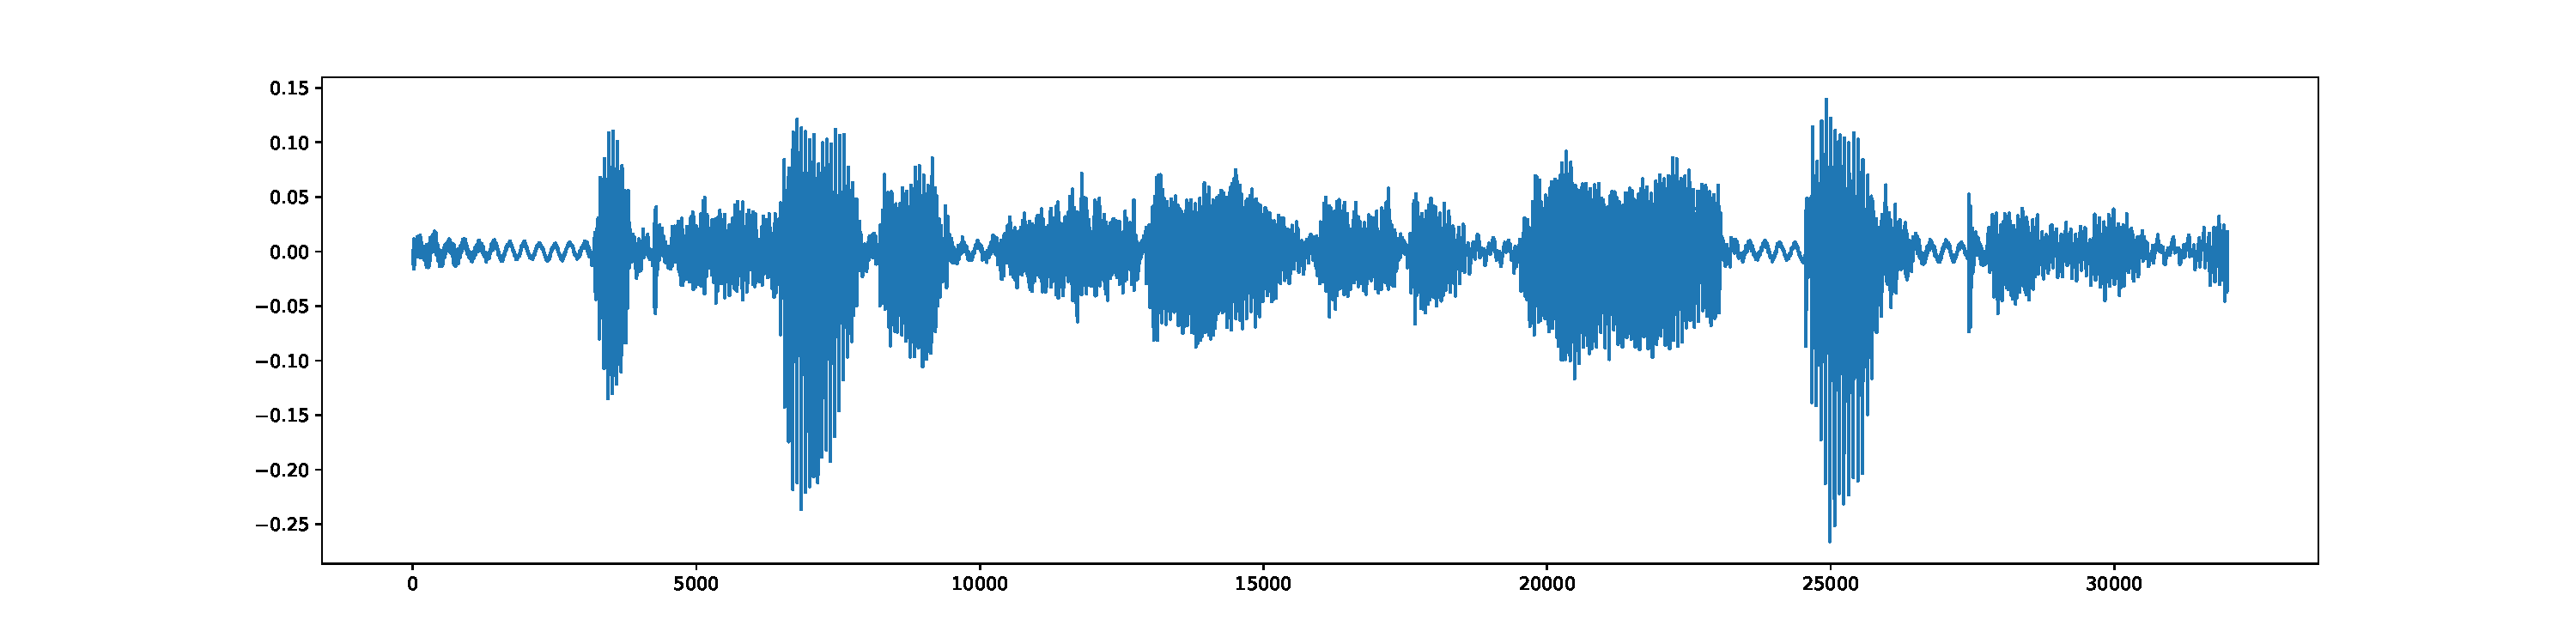
\includegraphics[width=1\textwidth]{Images/original_audio.pdf}
\caption{Original Waveform.}
\end{figure}

\begin{figure}[H]
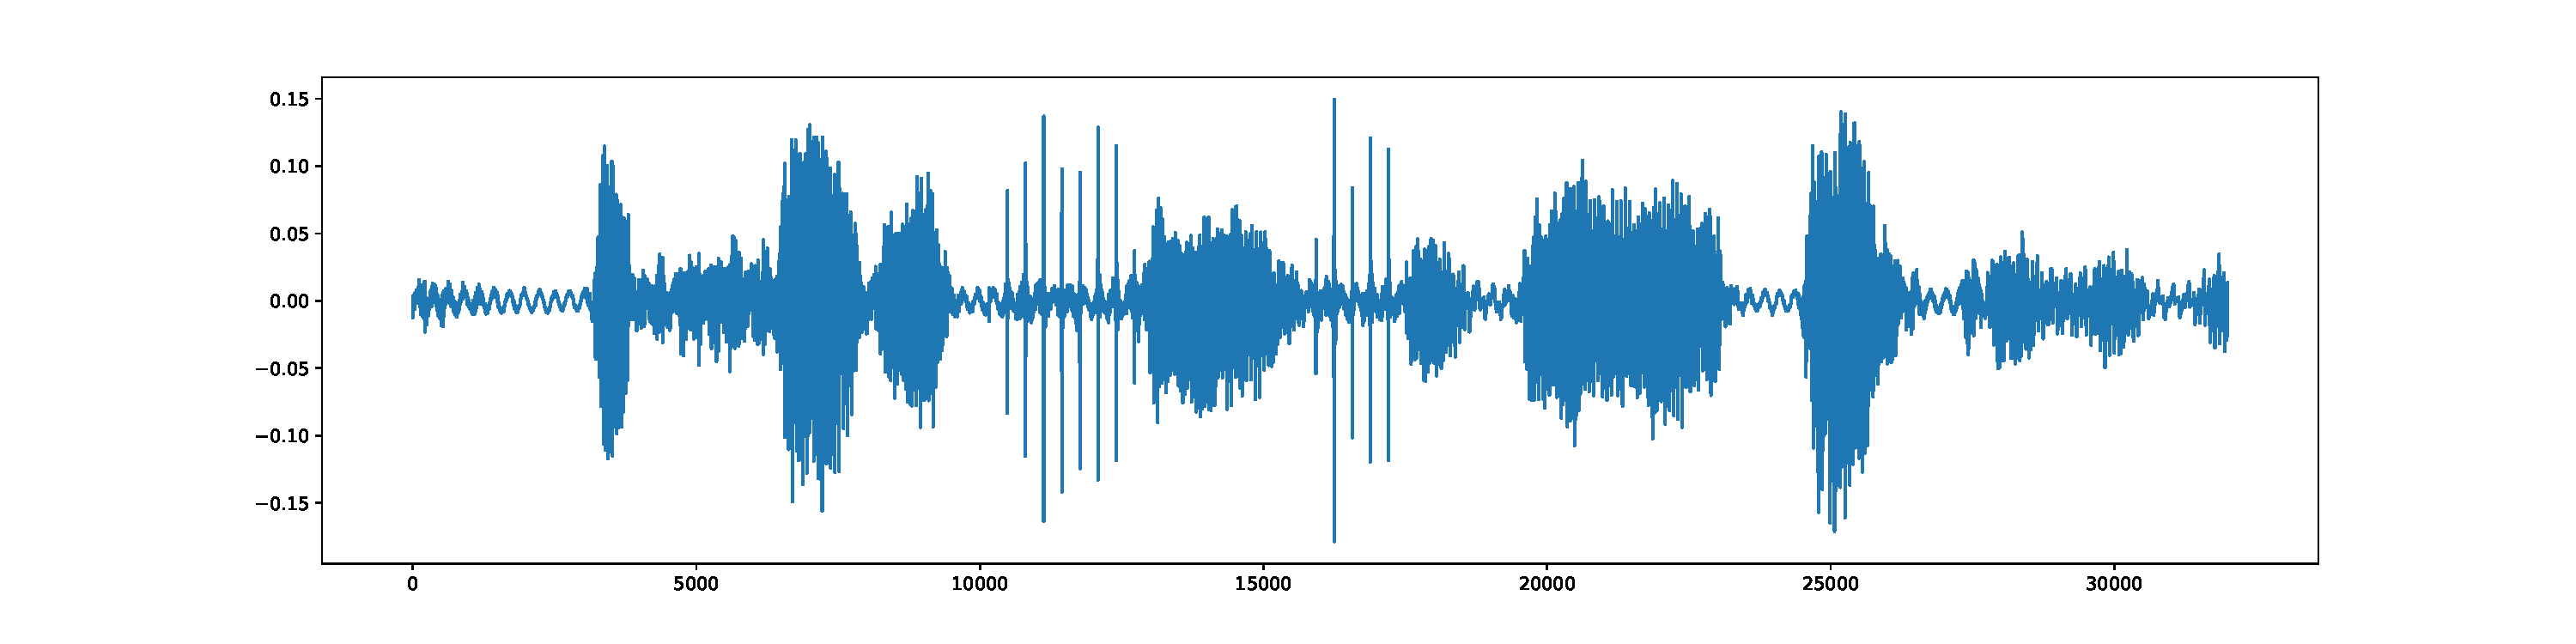
\includegraphics[width=1\textwidth]{Images/compressed_audio.pdf}
\caption{Reconstructed Waveform.}
\end{figure}

\chapter{Conclusion}
In conclusion, this project highlights the potential of deep learning-based audio codecs in enhancing compression efficiency and improving audio quality. The subjective evaluation conducted in this study shows that our Neural Audio Codec performs comparably to traditional audio codecs, Opus and EVS, at low bitrate despite being a relatively new approach to audio compression. By releasing open-source code and pre-trained models, this study provides a valuable resource for further research and improvement. Moreover, with the endless possibility of further advancements in deep learning-based audio synthesis and representation learning, there is a significant potential for improving audio codecs' efficiency and quality. The future of audio compression seems promising, and the development of deep learning-based models can play a pivotal role in it.
\addcontentsline{toc}{section}{References}
\renewcommand{\bibname}{References}
\bibliographystyle{plain}
\bibliography{ref}

\chapter{Appendices}
\textbf{Appendix A: Vector Quantization Compression Mechanism}\\
\begin{itemize}
  \item The encoder produces one embedding for e.g. 0.1s of audio
  \item A vector of length 3 encode in float16 use 3 * 16= 48 bits
  \item Per second: 48 * 10 = 480 bits
\end{itemize}
\begin{figure}[H]
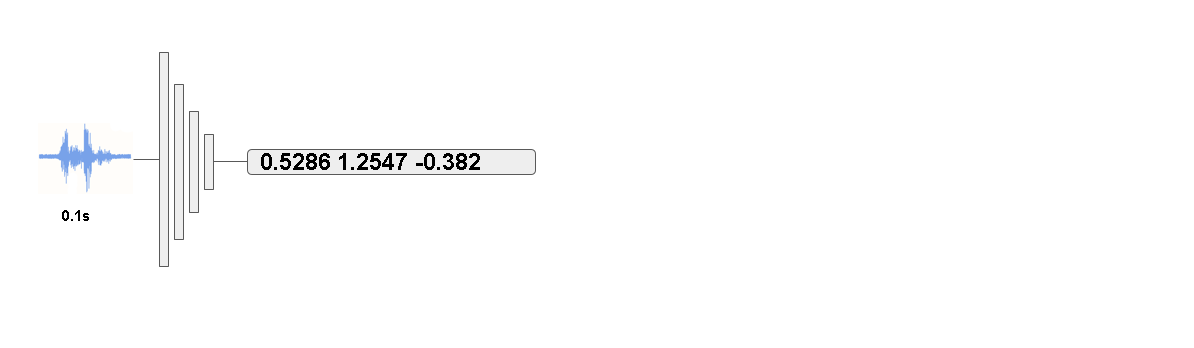
\includegraphics[width=1\textwidth]{Images/compress1.png}
\caption{Step I}
\end{figure}

\begin{itemize}
  \item A vector quantizer learns a fixed “dictionary” of template vectors (called code-words)
\end{itemize}
\begin{figure}[H]
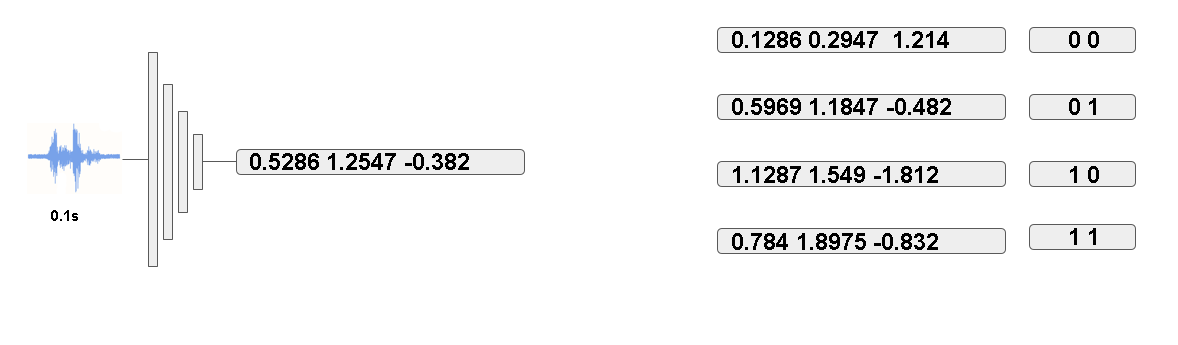
\includegraphics[width=1\textwidth]{Images/compress2.png}
\caption{Step II}
\end{figure}

\begin{itemize}
  \item We replace the embedding by its closest neighbor in the dictionary
\end{itemize}
\begin{figure}[H]
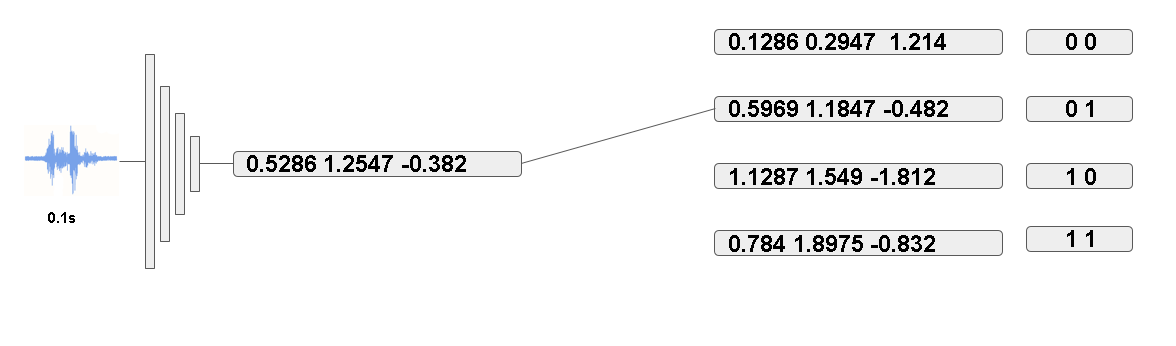
\includegraphics[width=1\textwidth]{Images/compress3.png}
\caption{Step III}
\end{figure}

\begin{itemize}
  \item Now we only need to transfer 2 bits (the index) to the receiver
\end{itemize}
\begin{figure}[H]
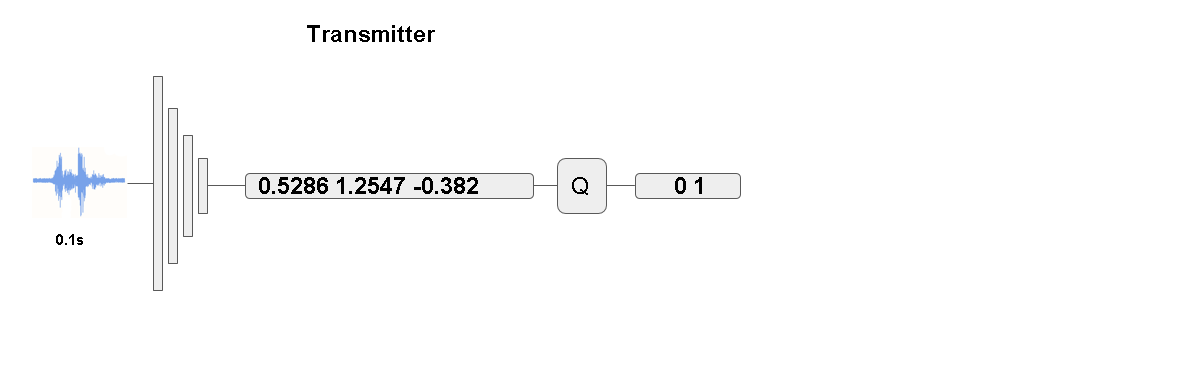
\includegraphics[width=1\textwidth]{Images/compress4.png}
\caption{Step IV}
\end{figure}

\begin{itemize}
  \item The receiver also has the codebook and uses it to retrieve the vector corresponding to the index
\end{itemize}
\begin{figure}[H]
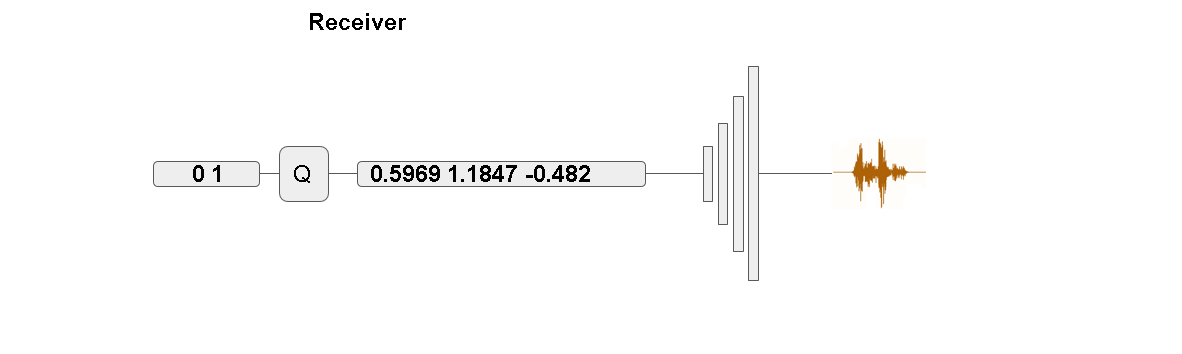
\includegraphics[width=1\textwidth]{Images/compress5.png}
\caption{Step V}
\end{figure}




\end{document}
